% TIK ŠĮ FAILĄ REIKIA KOMPILIUOTI

% ------------------------------------------------------------------------------
%                                   PREAMBLE                                  
% ------------------------------------------------------------------------------
\documentclass[a4paper, 12pt]{article}


% ---------------------------- PAGRINDINIAI PAKETAI ----------------------------

\usepackage[utf8]{inputenc}            % naudojama, kai .tex failas UTF-8 koduotės
\usepackage[L7x]{fontenc}              % nurodoma lietuviško teksto koduotė Latin-7
\usepackage[english, lithuanian]{babel}         % nurodoma, kad dokumentas yra lietuviškas

\usepackage{lmodern}                   % dokumente naudojamas šriftas Latin Modern
\usepackage{microtype}                 % optimizuojami atstumai tarp raidžių žodyje
\usepackage{indentfirst}               % atitraukiama pirmoji naujo skyriaus eilutė
\usepackage{icomma}                    % po kablelio skaičiaus viduryje nebus tarpo

\usepackage{amsmath, amssymb, amsthm}  % matematiniai simboliai ir konstrukcijos
\usepackage{mathtools}                 % standartinio AMS paketo amsmath išplėtimas
\usepackage{graphicx}                  % grafinių failų įterpimas ir kiti nustatymai
\usepackage{booktabs}                  % reikalingas tvarkingoms lentelėms sudaryti
\usepackage{caption}                   % paveiksliukų ir lentelių užrašų formavimas
\usepackage{geometry}                  % paraščių ir kitų lapo parametrų nustatymai
\usepackage{hyperref}                  % interaktyvioms nuorodoms dokumente sukurti

\usepackage{float}                     % for float enviroment positions
\usepackage{enumitem}                  % for lists customization

% ---------------------------- DOKUMENTO NUSTATYMAI ----------------------------

\geometry{left = 3cm, top = 2cm, right = 1.5cm, bottom = 2cm} % paketo geometry parametrų nustatymai
\linespread{1.5}                       % tarpas tarp eilučių

\captionsetup{                         % paketo caption parametrų nustatymai (paveiksliuku, lenteliu numeravimas)
    format = hang,                  
    labelfont = bf,             % žodžio pav, lentelė, ... teksto stylius
    textfont = footnotesize,    % caption teksto dydis
    justification = centering, 
    % skip = 0pt,               % atstumas iki paveiksliuko, lentelės, ...
    tablename = lentelė,        % caption pavadinimas prie table
    figurename = pav,           % caption pavadinimas prie figure
    labelsep = period           % atstumas tarp label (pav, ...) iki caption teksto
}

\hypersetup{                           % paketo hyperref parametrų nustatymai (linkai, citavimas)
    unicode = true,
    linktoc = all,
    linktocpage = false, 
    colorlinks = true,       % linkai yra spalvoti
    linkcolor = black,       % \ref color
    filecolor = Maroon, % \href{run:}{} color
    urlcolor = blue,         % url color
    citecolor = blue,        % \cite color          
    breaklinks = true 
    % pdfauthor = {Autorius},  % pdf dokumento meta-duomenys (autorius)
    % pdftitle = {Pavadinimas} % pdf dokumento meta-duomenyse (pavadinimas)
}

\graphicspath{{figures/}}    % paveikliuku folderis (kad būtų galima nurodyti tik pavadinimą)


% ----------------------- PAPILDOMI PAKETAI IR NUSTATYMAI -----------------------


\usepackage{pdfpages}		% pdf puslapių importavimui
\usepackage{titlesec}                  % leidžia keisti skyriaus pavadinimo stilių
\titlelabel{\thetitle.\quad}           % dedamas taškas po skyriaus numeriu tekste
\let\tocnumdot\numberline              % uždeda tašką po skyriaus numeriu turinyje
\def\numberline#1{\tocnumdot{#1.}} 

\usepackage{tocloft}                                  % format and control table of contents
\renewcommand{\cftsecleader}{\cftdotfill{\cftdotsep}} % for dots in sections toc 

\usepackage{bbm}                      % matematinio teksto ir simbolių formatavimas
\usepackage{xfrac}                    % display `small', nice fractions (alternative nicefrac)
\usepackage{siunitx}                  % SI vienetų paketas

% \setlength{\parindent}{0pt}            % no paragraph indention
% \setlength{\parskip}{1em}              % add spave between paragraphs

\newcommand{\subsubsubsection}[1]{\paragraph{#1}\mbox{}\\}  % sukuriamas \subsubsubsection, kuris numeruojamas
% \setcounter{secnumdepth}{4}
% \setcounter{tocdepth}{4}

%\usepackage[dvipsnames]{xcolor}           % papildomos spalvos
%\definecolor{back}{RGB}{245, 245, 245}    % nauja spalva (pilka, tinkanti kodo fonui)

\usepackage{algorithm}              % for writing algorithms
\usepackage[noend]{algpseudocode}   % for writing algorithms

\usepackage{verbatim}               % programinio kodo ir komentaru įterpimas
\usepackage{fancyvrb}               % programinio kodo įterpimas ir formatavimas
\usepackage{fvextra}                % programinio kodo formatavimas
\usepackage{listings}               % programinio kodo įterpimas ir formatavimas (galima naudoti caption)
\renewcommand{\lstlistingname}{išvestis} % lstlisting caption pavadinimas
\lstset
{ %Formatting for code in appendix (paprastas)
    basicstyle = \linespread{1}\tt\small,
    breakatwhitespace = false,
    breaklines = true,
    columns = fullflexible,
    showspaces = false,
    showstringspaces = false,
    showtabs = false,
    tabsize = 4,
    % aboveskip = 5pt,
    % belowskip = 5pt,
    inputencoding=utf8,
    escapeinside = {(*@}{@*)}
}

\usepackage{tabu, multirow} % lenteleje storesnes linijas padaryti, kelias eilutes apjungti
\usepackage{diagbox}

% Spalvoti TODO komentarai
\usepackage[colorinlistoftodos]{todonotes}
\newcommand{\TD}[1]{\todo[inline, color=red!40]{#1}}

% ------------------------- NELABAI REIKALINGI PAKETAI -------------------------
% --------------------------- BET GALI BŪTI NAUDINGI ---------------------------

\usepackage{multicol}                  % leidžia rašyti tekstą į kelis stulpelius
\usepackage{lipsum}                    % for dummy text only
\usepackage{titling}                   % for beutiful title
\usepackage{pifont}                    % special symbols 
\usepackage{physics}                   % for typesetting equations for physics
% \usepackage{subcaption}                % subcaption in figures (not working with subfig)
\usepackage{subfig}                    % for subfigures in figure 
\usepackage{wrapfig}                   % wrap text around figures 


\setlist[enumerate]{ % list formatting
    itemsep = 0.1pt,
    topsep = 5pt
}
\setlist[itemize]{ % list formatting
    itemsep = 0.1pt,
    topsep = 5pt
}

\lstdefinestyle{fancycode}{                        % aplinkos lstlisting nustatymai graziam kodo iterpimui:
                                                   % KODE REIKES NURODYTI [style=fancycode]
    backgroundcolor = \color{back},           % colour for the background
    commentstyle = \it\color{magenta},        % style of comments
    keywordstyle = \color{blue},              % style of keywords
    numberstyle = \tiny\color{black},         % style used for line-numbers
    stringstyle = \color{ForestGreen},        % style of strings
    basicstyle = \linespread{1}\footnotesize, % font size/family/etc. for source 
    breakatwhitespace = false,                % sets if automatic breaks should only happen at whitespaces
    columns = fullflexible,                   % for optimal spacing between characters
    keepspaces = true,                        % keep spaces in the code, useful for indetation
    breaklines = true,                        % automatic line-breaking       
    %captionpos = b,                          % position of caption (t/b)
    numbers = left,                           % position of line numbers (left/right/none)
    numbersep = 12pt,                         % distance of line-numbers from the code
    showspaces = false,                       % emphasize spaces in code 
    showstringspaces = false,                 % emphasize spaces in strings 
    showtabs = false,                         % emphasize tabulators in code
    tabsize = 2,                              % default tabsize
    frame = trBL,                             % showing frame outside code 
%                                             %(none/leftline/topline/bottomline/lines/single/shadowbox/trbl)
    escapeinside = {(*@}{@*)},                % specify characters to escape from source code to LATEX
    rulecolor = \color{gray},                 % Specify the colour of the frame-box
    frameround = fttt,                        % from top-right (t - round)
    %framerule = 2mm,                          % margin of frame
    inputencoding=utf8,
    aboveskip = 20pt,                         % space above 
    belowskip = 15pt                          % space below
}

\newcommand{\file}[1]{\href{run:#1}{#1}}   % komanda failo pavadinimui iterpti, kad ji galima butu atidaryti is pdf
\renewcommand{\eqref}[1]{\hyperref[#1]{\textbf{\footnotesize \ref{#1}}}} % kad eqref numerius boldintu

% \definecolor{black1}{RGB}{95, 95, 95}
% \renewcommand{\_}{{\color{black1} \underline{\hspace{0.35em}}}} % apatinis pabraukimas

% \usepackage{slantsc} % combine two font styles
% \newcommand{\textscit}[1]{\textsl{\textsc{#1}}} % small caps italic
\usepackage{newtxmath}
\usepackage[style=dutch]{csquotes}
\newcommand{\angstrom}{\textup{\AA}}
\def\UrlBreaks{\do\/\do-}

\begin{document}

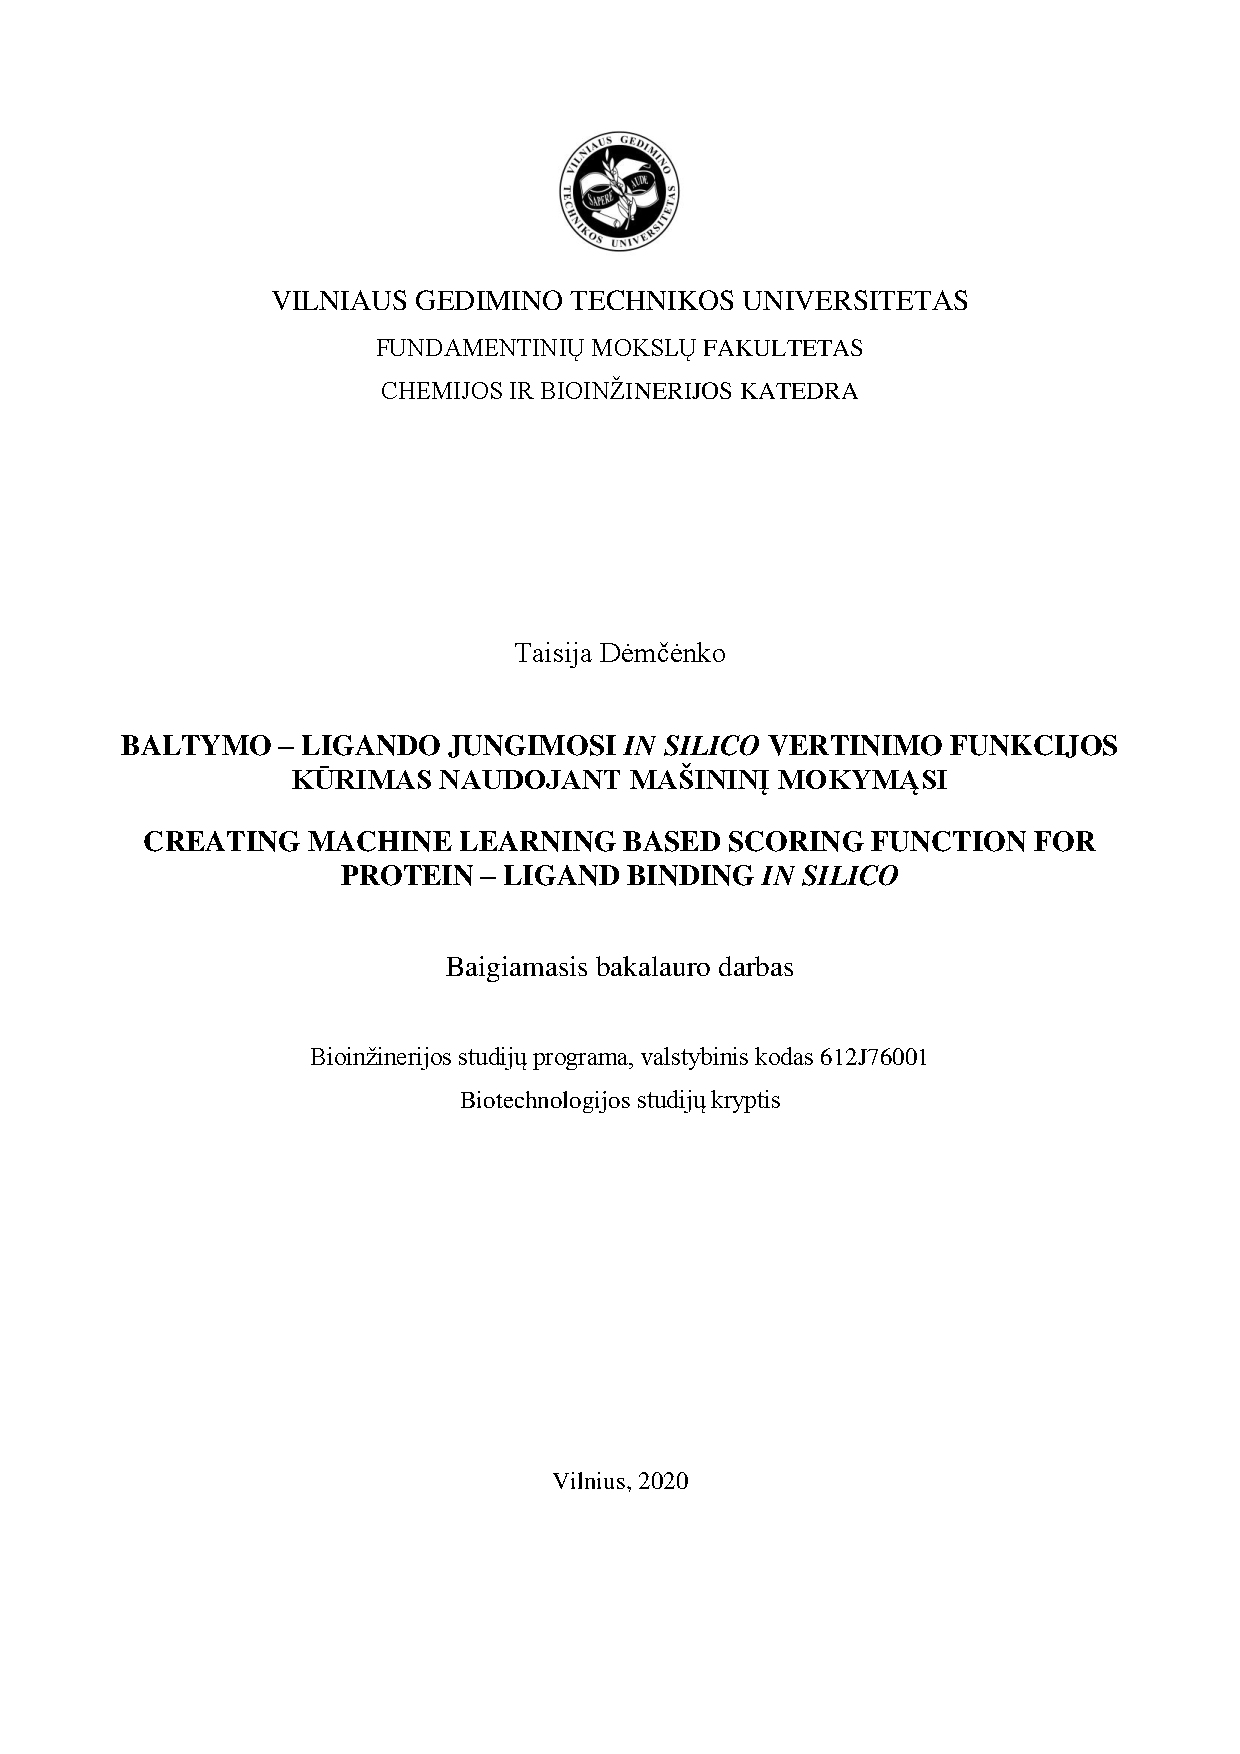
\includepdf[page={1}]{titulinis}
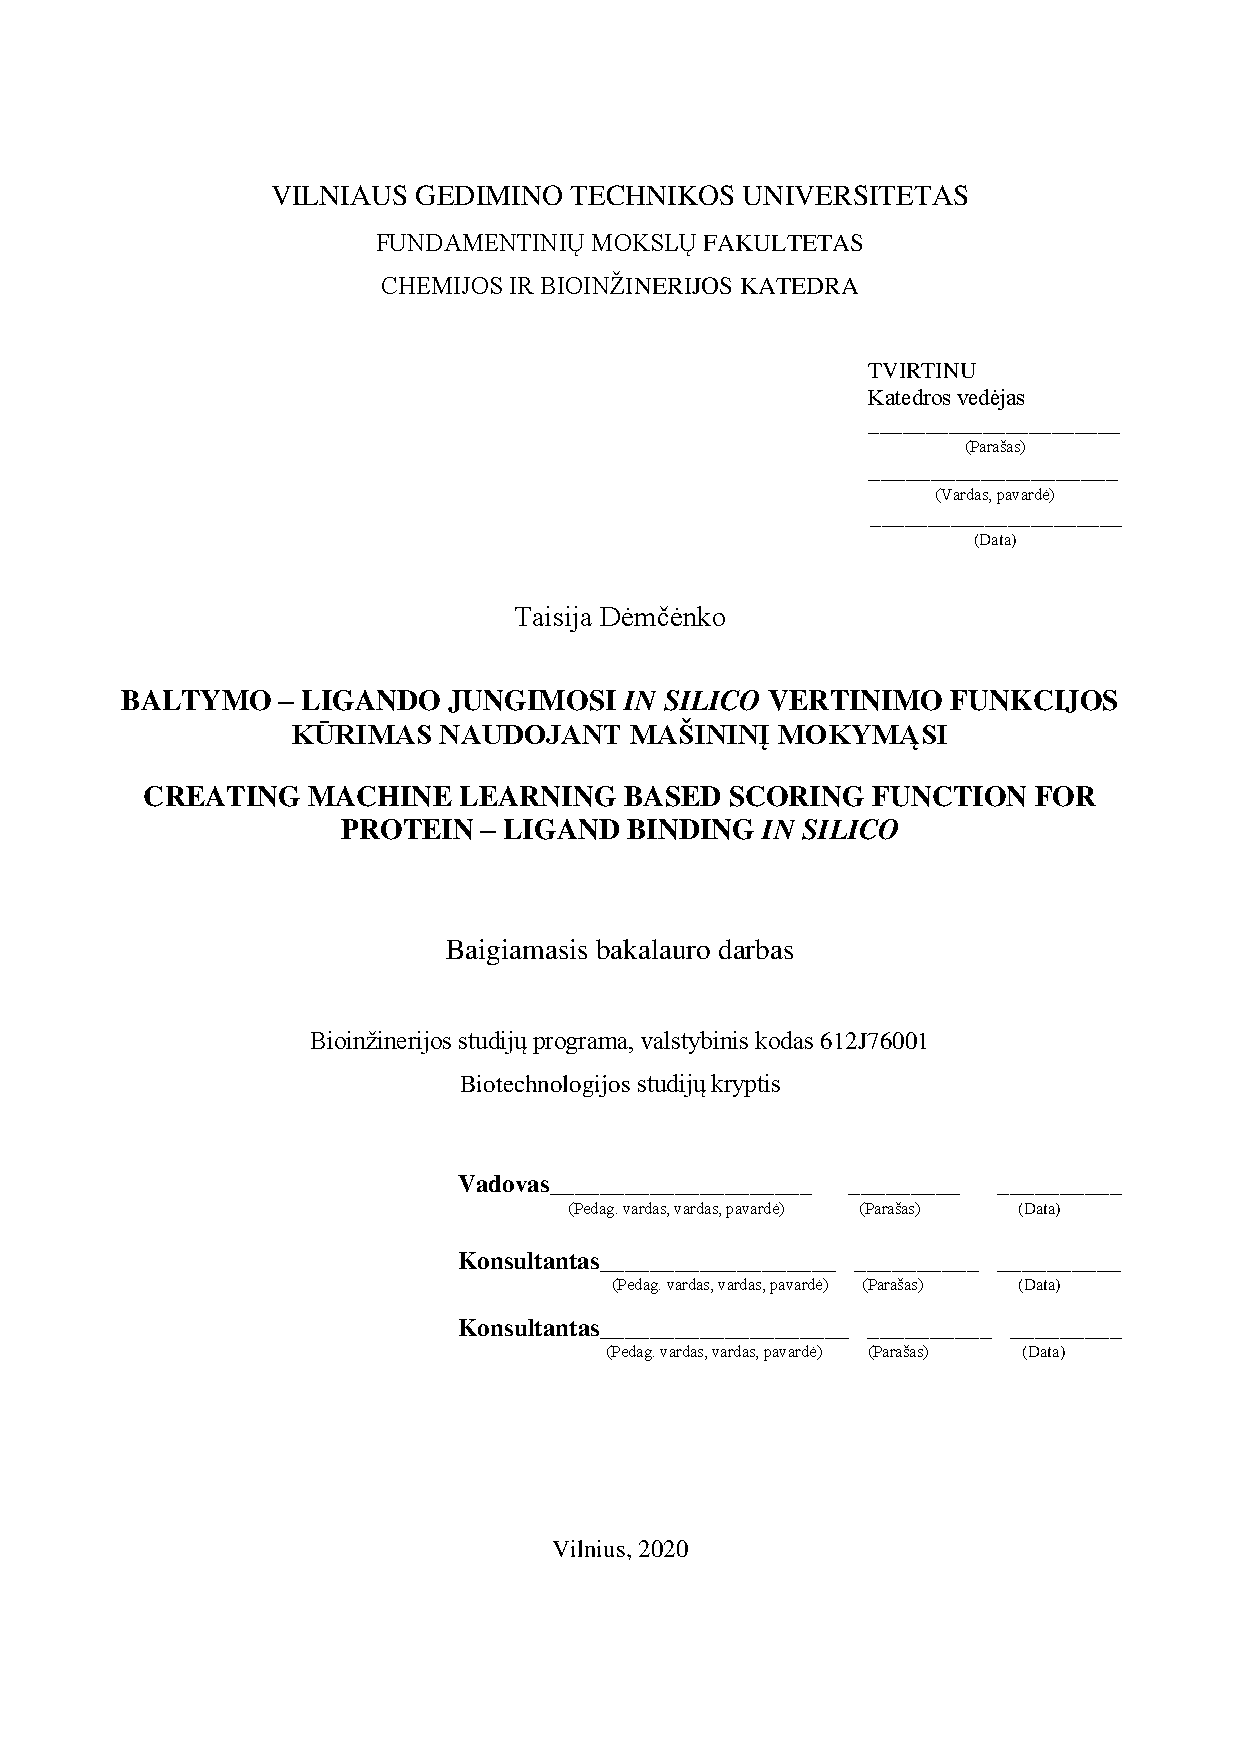
\includepdf[page={1}]{antras}

\tableofcontents
\pagebreak

%---------------------
%  ĮVADAS
%---------------------

\section*{ĮVADAS}
\addcontentsline{toc}{section}{ĮVADAS} 

Baltymo sąveikos su kitomis molekulėmis supratimas yra svarbus skirtingose biochemijos srityse, ypač farmacijos ir biofarmacijos srityse.\cite{hochuli_visualizing_2018}\cite{sethi_molecular_2019} Proteino--ligando kompleksų dėsnių suvokimas yra reikšmingas naujų vaistų atradimui - vaistai paprastai užima ligando vietą komplekse. Naujo vaisto kūrimas įprastai prasideda nuo didelės kolekcijos ligandų rinkimo; kiekvieną iš šių ligandų planuojama išanalizuoti \textit{in vitro} kaip potencialų vaistą. Aišku, tai reikalauja daug resursų ir laiko. Baltymo--ligando komplekso modeliavimas \textit{in silico} ir tolimesnė aktyvių ligandų virtuali atranka yra metodas, leidžiantis žymiai palengvinti naujo vaisto kūrimo procesą laiko ir kainos atžvilgiu. Šio metodu galima palyginus greitai išskirti molekules, turinčias didžiausią potencialą, vietoje pilnos kolekcijos analizės. \cite{berry_practical_2015}\cite{sethi_molecular_2019}

Sparčiai didėjanti skaičiavimo galia leidžia naudoti vis sudėtingesnius algoritmus baltymų modeliavimui bei jo surišimo su ligandu prognozavimui. Ypač gerus rezultatus parodo mašininio mokymosi algoritmai, nes dažnai nereikalauja papildomų žinių apart baltymo ir ligando molekulinės struktūros ir/ar fiziko--cheminių savybių. Tačiau mašininio mokymosi algoritmo rezultatus priklauso nuo turimų duomenų kiekiu ir kokybe: kuo duomenys kokybiškesni, tuo būna geresni tokių modelių rezultatai. Baltymų ir kitų junginių struktūrų ir parametrų duombazės nuolat pildosi naujais arba patobulintais duomenimis. Todėl kuriami vis nauji mašininio mokymosi modeliai, apmokinti ant dar išaugusios ir patobūlintos baltyminių kompleksų duombazės.\cite{meng_molecular_2011} Vienas toks modelis, paremtas dirbtiniu neuroniniu konvoliuciniu tinklu, bus pasiūlytas šitame darbe.

Šio darbo tikslas yra sukurti naują baltymo--ligando surišimo prognozavimo įrankį (vertinimo funkciją), pagrįstą mašininio mokymosi algoritmu. Šio darbo iškeliami uždaviniai:
\begin{enumerate}
\item Išanalizuoti jau sukurtas vertinimo funkcijas, kurios sprendžia tą patį problemą, ir išsirinkti vieną iš jų kaip atramos tašką.
\item Paruošti modelio kodą, išrinkti kokybišką baltymo--ligando kompleksų rinkinį ir apmokyti modelį naudojant šį rinkinį.
\item Įvertinti apmokyto modelio prognozavimo rezultatus ir palyginti su panašių modelių įvertinimais.
\end{enumerate}


% ----------------------------------------------------------------
%                         FAILŲ IMPORTAI                        
% ----------------------------------------------------------------

% !TEX root = referatas.tex

\section{LITERATŪROS APŽVALGA IR ANALIZĖ}

\subsection{Baltymų sąveikos su skirtingomis molekulėmis}

Baltymai yra didelės ir sudėtingos biologinės molekulės, atliekančios skirtingas funkcijas, tarp kurių yra katalizės funkcija. Tokie baltymai vadinami fermentais ir turi aktyvųjį centrą, prie kurio prisiriša kita molekulė; sudarytas kompleksas skatina arba slopina tam tikrą reakciją. Molekulė (ligandas) gali prisijungti vandenilinių ryšių, elektrostatinių ryšių, hidrofobinės sąveikos ar Van der Valso jėgų dėka.\cite{du_insights_2016} Šis surišimas paprastai yra trumpalaikis bei grįžtamasis. 

Veikiantys organizme baltymai būna tretinės arba ketvirtinės struktūros. Tretinė struktūra yra baltymo kompaktiškas susilankstymas erdvėje su skirtingų ryšių (disulfidinių, vandenilinių bei kitų) pagalba. Baltymo struktūrą galima nustatyti skirtingais metodais (rentgenostruktūrine analize, branduolių magnetinio rezonanso metodu ir t.t.),\cite{du_insights_2016} ir nustatytos struktūros yra renkami į duombazes (pvz. PDB). Tačiau to neužtenka proteino--ligando sąryšio prognozavimui: reikia dar nustatyti aktyvaus centro vietą ir nustatyti, ar jis gali pririšti pasirinktą ligandą. Fermentai turi didelį specifiškumą - jie geba atrinkti tik vieną specifinę molekulę iš milijonų skirtingų substratų.

Aktyvusis centras paprastai užima tik 10--20 \% baltymo masės, tačiau yra svarbiausia fermento dalis. Jis dažniausiai yra sudarytas iš 3--4 aminorūgščių, prie kurių jungsis ligandas.\cite{du_insights_2016} Skirtingų fermentų atvejais tai gali būti mažos molekulės, nukleorūgštys arba kiti baltymai ir peptidai. Šiame darbe bus analizuojami tik baltymo ir mažos molekulės kompleksai.

Ankstesnė baltymo--ligando komplekso \enquote{spynos ir rakto} teorija teigė, kad ligandas privalo turėti tą patį dydį ir formą, kaip ir baltymo aktyvaus centro kišenė. Tačiau eksperimentiniu būdu buvo nustatyta, kad susiriša kompleksai, kurių molekulių formos nepilnai sutampa.\cite{du_insights_2016} Todėl išsivystė naujesnė \enquote{indukuoto įtalpinimo} teorija, kuri teigia, kad priartėjęs ligandas keičia baltymo aktyvaus centro struktūrą, taip pat gali ir pats nežymiai pasikeisti. Tačiau net to neužtenka, nes abi teorijos neatsižvelgia į pačio baltymo dinamiškumą. Baltymai nuolat keičia savo konformaciją skirtingose aplinkose; tik būdami specifinėje konformacijoje, baltymas gali surišti specifinį ligandą. Taip teigia naujausia \enquote{konformacijos išrinkimo} teorija. Šios trys teorijos nepaneigia viena kitos - skirtingose atvejuose buvo eksperimentiškai nustatyti visų trijų mechanizmų surišimai.\cite{du_insights_2016}

\subsubsection{Baltymo su ligandu surišimo konstanta}

Galima pavaizduoti baltymo--ligando komplekso sudarymą šia pusiausvyros lygtimi:

\begin{equation}
L + P \xrightleftharpoons[K_{off}]{K_{on}} LP
\end{equation}

kur L - ligandas, P - baltymas, LP - baltymo--ligando kompleksas, $K_{on}$ ir $K_{off}$ - surišimo ir disocijavimo reakcijų kinėtinės konstantos.\cite{du_insights_2016}

Nors baltymo--ligando jungimosi prognozavimo algoritmai paprastai prognozuoja, ar vyks surišimas, prognozavimui naudojama ne surišimo konstanta $K_{b}$, o atvirkštinė jai disociacijos konstanta $K_{d}$. Ji priklauso nuo visų trijų koncentracijų:

\begin{equation}
K_{d} = \frac{1}{K_{b}} = \dfrac{[L][P]}{[LP]} = \frac{K_{off}}{K_{on}}
\end{equation}

Pusiausvyros konstantos vienetai yra M (g/mol).

Zubrienė ir Matulis \cite{matulis_carbonic_2019} aprašo skirtumą tarp stebimos ir tikros surišimo konstantos. Jie atkreipia dėmesį į tai, kad baltymas gali egzistuoti keliose konformacijose, tarp kurių tik viena gali susirišti su ligandu. Baltymo konformacijos pakeitimas gali reikalauti nemažai energijos, ir jei tirpale yra daugiau neaktyvios baltymo konformacijos, išmatuota $K_{d}$ parodys tikros surišimo konstantos ir konformacijos keitimui reikalingos energijos sumą. Tikra surišimo konstanta bus aukštesnė. Taip pat autoriai pabrėžia, kad stebima $K_{d}$ priklauso nuo tirpalo pH, tuo metu tikroji $K_{d}$ nepriklauso. Tą reikia turėti omenyje renkant duomenis mašininio mokymosi modeliui, nes tai gali paveikti modelio prognozių tikslumą.

Kitas svarbus aspektas yra vandens molekulių koordinatės baltymo struktūroje. Straipsniuose \cite{berry_practical_2015} ir \cite{schiebel_intriguing_2018}  autoriai kalba apie vandens ypatingą svarbumą proteino surišimui su ligandu. Proteinai \textit{in vivo} yra apsupti vandens molekulėmis, kurios veikia baltymo konformaciją bei dalyvauja komplekso surišime. Straipsnio autoriai nurodo, kad vandeniui skiriama per mažai dėmesio, nes ji atlieka daug sudėtingų funkcijų, o dėl to dažnai sunku prognozuoti surišimo stiprumą, net kai yra nustatyta baltymo struktūra. Apie tai rašo ir Sethi et al.\cite{sethi_molecular_2019}; jie pabrėžia, kad informacijos apie vandens molekules yra per mažai dėl vandenilio koordinačių trukumo rentgeno-struktūriniu būdu nustatytose baltymų kristalinėse struktūrose, bei patikimų teoretinių žinių apie vandens ir ligando sąveiką nepakankamumo. Iš kitos pusės, Chen et al.\cite{chen_hidden_2019} parodo, kad vandenio molekulių įvedimas į struktūras nepagerino aprašomo modelio prognozavimo tikslumo. Šiame darbe vandeniui nebus skirta dėmesio.

\subsection{Ligando įvedimas į baltymą}

Ligando įvedimas į baltymą (angl. \textit{molecular docking}) yra molekulių projektavimo technika. Šios technikos esmė yra naudojant baltymo ir ligando erdvines struktūras, rasti tokias molekulių padėtis, kad susijungus kompleksui šiose padėtyse, ryšys būtų kuo stipresnis. Ligando įvedimo į baltymo technika sprendžia du uždavinius: ligando pozicijų aktyviajame centre prognozavimas, ir tos pozicijos surišimo su baltymu stiprumo įvertinimas.\cite{ain_machine-learning_2015}\cite{ballester_does_2014} Antra uždavinį atlieka vertinimo funkcija (angl. \textit{scorinc function}).\cite{berry_practical_2015} Sethi et al.\cite{sethi_molecular_2019} aprašo skirtingus pozicijų paieškos bei vertinimo funkcijų algoritmus, taip pat pateikia daug jų pritaikymo pavyzdžių.

Pagrindinė ligando įvedimo į baltymą technikos problema yra ta, kad reikia ištirti labai didelį skaičių galimų susijungimo variantų.\cite{huang_advances_2010} Ankstesniais laikais tokius tyrimus smarkiai ribojo kompiuteriniai resursai, tačiau dabar kompiuteriai yra pajėgesni. Šiuo metu yra sukurta nemažai programinės įrangos baltymo ir ligando prijungimui modeliuoti, tarp kurių yra ir nemokamai ir viešai prieinamų, tokių kaip \enquote{AutoDock} bei \enquote{LeDock}.\cite{wang_comprehensive_2016} Verta paminėti, kad projektavimui pagreitinti yra naudojami supaprastintos struktūros arba molekuliniai vektoriai (angl. \textit{molecular fingerprints}).\cite{ballester_does_2014}

\subsubsection{Ligando pozicijos komplekse paieškos algoritmai}

Kaip jau buvo minėta, reikia ištirti labai didelį ligando pozicijų kiekį. Analizės greitinimui buvo sugalvoti skirtingi kompiuteriniai algoritmai. Juos galima klasifikuoti pagal ignoruojamų parametrų kiekį. Pats paprasčiausias algoritmas atkreipia dėmesį tik į baltymo bei ligando nelanksčias trimates struktūras. Toks algoritmas ieško ligando pozicijas, kurios atitinka \enquote{spynos ir rakto} teorijai.\cite{du_insights_2016} Sudėtingesnis algoritmas, vadinantis inkrementiniu konstravimu (angl. \textit{incremental construction}), fragmentuoja ligandą palei jo galinčius suktis ryšius į segmentus.\cite{huang_advances_2010} Dar vienas algoritmas vadinamas genetiniu: pasirenkama ligando pozicijų grupė ir įvertinamos jų surišimo su baltymu konstantos, toliau geriausios pozicijos atsitiktinai nežymiai pakeičiamos ir/ar fragmentai pozicijų sumaišomos tarpusavyje, ir taip atsiranda sekanti pozicijų \enquote{populiacija}. Procesas kartojasi daug kartų. Kituose straipsniuose\cite{huang_advances_2010}\cite{wang_comprehensive_2016} pozicijos paieškos algoritmus dalinama į tris grupes: formų priderinimo (angl. \textit{shape matching}), sistematinės paieškos (angl. \textit{systematic search}) ir stochastinės paieškos (angl. \textit{stochastic search}) algoritmai.

% two rigid molecules - only protein ir rigid - two molecules are flexible

\subsubsection{Komplekso surišimo vertinimo funkcijos}

Vertinimo funkcija yra antras ligando įvedimo į baltymą etapas: naudojant vertinimo funkciją, galima prognozuoti baltymo ir turimos pozicijos ligando surišimą (arba disociacijos konstantą, $K_{d}$). Gera vertinimo funkcija turi būti didesnio nei 1 $pK_{d}$ tikslumo, greitai ir lengvai skaičiuojama. Berry et al.\cite{berry_practical_2015} vadina vertinimo funkcijas silpnąja baltymo--ligando jungimosi vieta, nes tai yra svarbiausia ligando įvedimo į baltymą dalis, kurioje iki šiol yra aptinkama nemažai problemų. 

Klasikinės vertinimo funkcijos skirstomos į tris grupes: funkcijos pagrįstos fizine sąveika, empirinės funkcijos ir funkcijos pagrįstos teorinėmis žiniomis.\cite{liu_classification_2015} Neseniai atsirado dar vienas vertinimo funkcijų tipas, kurį dažniausiai vadina kaip mašininio mokymosi vertinimo funkcijos. Jos parodo geresnius rezultatus baltymo--ligando jungimosi prognozavimee.\cite{wojcikowski_performance_2017} Liu et al.\cite{liu_classification_2015} rekomenduoja šį tipą vadinti deskriptorių funkcijomis (angl. \textit{descriptor-based}), argumentuojant tuo faktu, kad terminas \enquote{mašininis mokymasis} aprašo ne teorinę bazę, bet technologiją. Kitas jų argumentas nurodo, kad teorinėmis žiniomis pagrįstos funkcijos taip pat gali naudoti mašininį mokymąsi. 

Vertinimo funkcijos rezultatų atitikimas tikrovei gali būti patikrintas vertinant pačią vertinimo funkciją. Tai daroma tikrinant funkcijos baltymo--ligando kompleksų surišimo prognozes su tikromis tų kompleksų vertėmis, paduodant funkcijai jau išanalizuotų kompleksų rinkinį. Huang et al.\cite{huang_scoring_2010} aprašo skirtingas vertinimo funkcijos įverčių formules. Viena iš klasikinių formulių yra šaknies vidurkio kvadrato nuokrypis (angl. \textit{root mean square deviation}). Jis skaičiuojamas tarp geriausios prognozuotos ligando pozicijos ir eksperimentiškai nustatytos pozicijos ir užrašomas taip:

\begin{equation}
RMSD(v, w) = \sqrt{\frac{1}{n} \sum_{i=1}^{n} {|| v_i - w_i ||}^2}
\end{equation}

kur $v_i$ ir $w_i$ yra du koordinačių rinkiniai, o $n$ yra atomų skaičius. Jeigu RMSD reikšmė yra mažesnė arba lygi 2\AA , prognozė laikoma sėkminga.\cite{berry_practical_2015} Didžiausias RMSD privalumas yra paprastumas, tačiau pagrindinė jo problema yra tame, kad maži ar simetriški ligandai turės mažą RMSD įvertį net nebūdami tinkamoje pozicijoje. Todėl buvo pasiūlyti keletas panašių įverčių kaip reliatyvaus poslinkio paklaida (angl. \textit{relative displacement error}), sąveika paremta tikslumo klasifikacija (angl. \textit{interaction-based acuracy classification}) ir kiti.\cite{huang_scoring_2010} Visi jie įvertina prognozuotos ligando pozicijos tinkamumą lyginant su duota pozicija.

Kita svarbi vertinimo funkcijos savybė yra nustatyti jungties stiprumą - tai yra atliekama regresijos būdu. Tam naudojama Pearson koreliacija tarp apskaičiuotų balų ir eksperimentinių duomenų.\cite{ain_machine-learning_2015} Ji turi sekančią formulę:

\begin{equation}
R_p = \frac{\sum_{k=1}^{N} (x_k - \langle x \rangle)(y_k - \langle y \rangle)}{\sqrt{[\sum_{k=1}^{N} (x_k - \langle x \rangle)^2][\sum_{k=1}^{N} (y_k - \langle y \rangle)^2]}}
\end{equation}  

kur $N$ yra kompleksų skaičius, $x_k$ -- eksperimentiškai nustatyta jungties energija, $y_k$ -- jungties energija apskaičiuota k-ajam kompleksui.\cite{huang_scoring_2010}

Toks $R$ įvertis yra aritmetinis visų kompleksų vidurkis. Šiam įverčiui pagerinti buvo pasiūlytas Spearman koreliaijos koeficientas, kurį apibūdina ši formulė:

\begin{equation}
R_s = 1 - \frac{6 \sum_{k=1}^{N} d_k^2}{N(N^2 - 1)}
\end{equation} 

Čia $d_k$ yra dviejų vertinimų skirtumas k-ajam kompleksui.

Trečioji svarbi vertinimo funkcijos savybė yra gebėjimas atrinkti tinkamus ligandus iš didelės jų gausos, kas dar vadinama virtualia atranka. Vienas iš šio proceso įverčių yra praturtinimo testas (angl. \textit{enrichment test}). Jis yra populiarus dėl savo paprastumo,\cite{ain_machine-learning_2015}\cite{wojcikowski_performance_2017} o jo formulė atrodo taip:

\begin{equation}
EF_{x\%} = \frac{\frac{\text{aktyvieji ligandai}(x\%)}{\text{visi ligandai}(x\%)}}{\frac{\text{aktyvieji ligandai}(100\%)}{\text{visi ligandai}(100\%)}}
\end{equation}

Kuo didesnis praturtinimo įvertis, tuo geresnė vertinimo funkcija. 

Kitas įvertis, taikomas klasifikacijos metodams, yra plotas po kreive (angl. \textit{area under curve} arba sutrumpintai AUC), kur kreivė yra ROC (angl. \textit{receiver operating characteristic}) kreivė. Jis parodo, ant kiek modelis geba atskirti aktyvius ir neaktyvius ligandus, kur AUC~=~0,5 reiškia visiškai atsitiktinus spėjimus, o AUC~=~1 reiškia idealų modelį. Šis metodas tinka, jei aktyvių ir neaktyvių ligandų skaičius rinkinyje yra maždaug panašus.\cite{huang_scoring_2010}

Vertinimo funkcijos patikrinimas dažnai vyksta naudojant kompleksus--\enquote{apgavikus} (angl. \textit{decoys}). Jie yra panašūs į realus aktyviai surištus kompleksus, tačiau iš tikrųjų nėra (arba bent jau neturi būti) aktyvūs. Populiariausios \enquote{apgavikų} duomenų bazės yra \enquote{DUD} (angl. \textit{A Directory of Useful Decoys}) bei \enquote{DUD-E} (angl. \textit{A Database of Useful Decoys: Enhanced}).\cite{berry_practical_2015} Tokie kompleksai yra generuojami kompiuteriniais metodais, dėl ko gali atsirasti šališkumas (angl. \textit{bias}), kaip teigia Reau et al.\cite{reau_decoys_2018} Šis šališkumas gali neigiamai paveikti ypač neuroniniu tinklu pagrįstos vertinimo funkcijos veikimą, nes tokios funkcijos savarankiškai atranda kompleksų klasifikacijos parametrus. Tokio šališkumo pavyzdys yra pateiktas straipsnyje\cite{chen_hidden_2019}, kurio autoriai teigia, kad \enquote{DUD-E} duombazėje yra analoginis šališkumas (angl. \textit{analogue bias}), dėl ko neuroninio tinklo vertinimo funkcijos gauna ypač aukštus įverčius (AUC~>~0,9). Autoriai paruošė konvoliucinių neuroninių tinklų modelį ir apmokė jį naudojant du skirtingus rinkinius: pilnus kompleksus ir tik vienus ligangus iš \enquote{DUD-E}. Rezultatai buvo labai panašūs ir abu gavo aukštą AUC įvertį, kas parodė, jog modelis klasifikuoja kompleksus neskiriant jokio dėmesio į baltymo receptoriaus struktūrą. Todėl autoriai siūlo stengtis nenaudoti kompiuteriu sugeneruotus \enquote{apgavikus}, o geriau naudoti eksperimentiškai analizuotus neaktyvius kompleksus. 

%-------------------------------------------------
%       MAŠININIS MOKYMAS
%-------------------------------------------------

\subsection{Mašininio mokymosi taikymas}

Mašininio mokymosi algoritmai pasižymi tuo, kad įgauna savo funkcionalumą mokymosi metu ir pati atranda dėsningumus, kurių žmogui būtų sunku ir per ilgai nustatyti.\cite{stepniewska-dziubinska_development_2018} Iš kitos pusės, mašininio mokymosi funkcijos pasirinktų parametrų esmė ne visada yra žmogui suprantama. Šis efektas dar vadinasi \enquote{juodos dėžės} efektu (angl. \textit{\enquote{black box}}) ir dažniausiai pasireiškia taikant dirbtinius neuroninius tinklus.\cite{liu_classification_2015} Mašininis mokymasis gali būti prižiūrėtas arba ne (angl. \textit{supervised} ir \textit{unsupervised}). Pirmu atveju funkcijai yra nurodoma, ar mokymosi metu gautas rezultatas atitinka tikrovei, ir naudojant šią informaciją, funkcija keičia savo parametrus kad padidintų tikslumą. Neprižiūrėto mokymosi atveju, funkcija bando pati klasifikuoti turimus duomenis į grupes pagal parametrus, kuriuos pati pasirenka.\cite{schmidhuber_deep_2015} Baltymo--ligando komplekso surišimo vertinimo atveju, mašininis mokymasis turi būti prižiūrėtas.

Mašininio mokymosi algoritmas gali spręsti klasifikacijos arba regresijos problemą.\cite{lehr_playing_2017} Klasifikacijos problemos pavyzdys būtų diagnozės išvedimas žinant tam tikrus parametrus - pavyzdžiui pacientų skyrimas į sergančius ir nesergančius pagal medicininės analizės rezultatus. Tuo metu regresijos problema yra susieta su tam tikro skaičiaus keitimu, o tokios problemos pavyzdys yra butų kainų prognozavimas. Prognozuojant komplekso $K_{d}$, galima taikyti abu sprendimus: klasifikacijos atveju tai būtų tiesiog ligandų sužymėjimas, parodantis ar jie susiriš su baltymų; regresijos atveju būtų bandoma prognozuoti tikslią $K_{d}$ vertę. Atitinkamai, klasifikuojančiai funkcijai užteks duombazės, kur yra pateikti galintys ir negalintys susirišti kompleksai (tam dažnai naudojami kompleksai--\enquote{apgavikai}). Tuo metu regresijos funkcijai bus reikalinga kompleksų duombazė su nustatytomis $K_{d}$ reikšmėmis.

\subsubsection{Dirbtiniai neuroniniai tinklai}
\label{sec:neuroniniai_tinklai}

Dirbtiniai neuroniniai tinklai yra mašininio mokymosi algoritmai, paremti gamtiniais neuroniniais tinklais.\cite{ragoza_proteinligand_2017} Dirbtinis neuroninis tinklas sudarytas iš neuronų sluoksnių, kurių būna du ir daugiau ir jie nuosekliai sujungti. Išoriniai sluoksniai yra \enquote{matomi}, o kiti sluoksniai yra paslėpti tarp jų ir vadinasi giliaisiais.\cite{schmidhuber_deep_2015} Ryšiai tarp neuronų turi svorius, kurie parodo to ryšio savotišką svarumą. Neuronai gali atlikti skirtingus pakeitimus ir būna įvairiai sujungti priklausant nuo tinklo tipo ir uždavinio. Neuroninių tinklų uždaviniai gali būti tam tikro \enquote{rašto} identifikavimas, signalo apdorojimas ir kiti, o galinis neuronų sluoksnis generuoja \enquote{atsakymą} - dažniausiai tai būna paduotos į tinklą informacijos klasifikavimas.\cite{ragoza_proteinligand_2017}

Kaip buvo paminėta, euroninis tinklas sudarytas iš daugelio neuronų. Kiekvienas neuronas gauna kelias įvestis, kiekviena iš kurių turi savo svorį. Iš pradžių svorio reikšmės yra parenkamos atsitiktiniu būdu, tačiau keičiamos modeliui besimokant. Neurono produkto skaičiavimo formulė atrodo taip:
\begin{equation}
z=\sum_{j=1}^{k} x_{j} w_{k}+b w_{0}
\end{equation}
kur $w_k$ yra tam tikros įvesties svoris ir $b$ yra nuolydis (angl. \textit{bias}). Nuolydis yra papildoma įvestis, kurios reikšmė yra fiksuota. Jis yra svarbus modelio lankstumui.

Dirbtinio neuroninio tinklo ypatumas yra tame, kad žmogus gali logiškai interpretuoti tik pirmą ir paskutinį tinklo sluoksnius. Paprasčiausi neuroniniai tinklai turi tik du sluoksnius, tačiau dabar populiarėja gilieji neuroniniai tinklai (angl. \textit{Deep Neural Networks}), kurie gali turėti daugiau nei tris sluoksnius. %Kaip būtent daugiasluoksnio neuroninio tinklo modelis atpažįsta tam tikrus požymius, iki šiol nėra tiksliai nustatyta. Iš to yra iškeliama svarbi problema: nesuprantama iki galo, kaip būtent veikia dirbtiniai neuroniniai tinklai. Šis efektas, kaip buvo minėta anksčiau, vadinamas \enquote{juodosios dėžės} efektu. Nepaisant to, 
Gilieji neuroniniai tinklai plačiai naudojami bioinformatikoje.\cite{chen_hidden_2019}\cite{stepniewska-dziubinska_development_2018}

Šiuo momentu egzistuoja daug skirtingų neuroninio tinklo išsidėstymų, pavyzdžiui rekursiniai (angl. \textit{recurrent neural network}) arba konvoliuciniai (angl. \textit{convolutional network}). Rekursinis tinklas turi neuronus, kurie savo išeinantį signalą vėl gauną praėjus fiksuotam laiko tarpui. Tai yra naudinga tyrinėjant sistemas, kur svarbu išlaikyti kontekstą (pavyzdžiui darbui su tekstu, kur prieš tai buvę žodžiai ir sakiniai yra reikšmingi sekančio žodžio prasmei). Šis principas buvo dar patobulintas ir 1997 m. išrastas ilgos trumpos atminties algoritmas (angl. \textit{long short-term memory}), kurio elementai gali nuspręsti, ar verta laikyti tam tikrą reikšmę neurono atmintyje. Rekursiniai tinklai ir natūralios kalbos apdorojimas (angl. \textit{natural language processing}) buvo analizuoti Jastrzębski et al.\cite{jastrzebski_learning_2018} kaip būdas spręsti bioinformatikos klasifikacijos problemas, kai duomenys apie molekules pateikiami SMILES formatu.

\subsubsection{Konvoliuciniai neuroniniai tinklai}

Konvoliuciniai neuroniniai tinklai dažniausiai naudojami paveikslėlių atpažinimui. Jie gali \enquote{atpažįsti} tam tikrus požymius (linijas, figūras, spalvas ir t.t.) ir pagal jas klasifikuoti paveikslėlį. Taip pat konvoliuciniai neuroniniai tinklai gerai tinka analizuoti daugiamates struktūras, pavyzdžiui baltymo molekulės struktūrą, ir yra perspektyvūs ligando įvedimo į baltymo vertinimui.\cite{hochuli_visualizing_2018} Ragoza et al.\cite{ragoza_proteinligand_2017} sėkmingai panaudojo konvoliucinį neuroninį tinklą baltymo--ligando kompleksų surišimo vertinimui. Jie aprašo konvoliucinių tinklų veikimo principą: kiekvienas tinklo sluoksnis bando atpažinti paveikslėlyje tam tikrą figūrą, ir kuo daugiau tinklas turi sluoksnių, tuo sudėtingesnius \enquote{raštus} jis gali identifikuoti ir klasifikuoti. Daugiau apie konvoliucinių neuroninių tinklų taikymą vertinimo funkcijose yra kalbama \ref{sec:vertinimo_funkciju_pavyzdziai} skyriuje.

Konvoliucinio neuroninio tinklo pirmas sluoksnis yra atsakingas už tiesinį duomenų transformavimą. Pasirenkamas filtro branduolys (angl. \textit{kernel}), tai yra svorių matrica. Filtro branduolys juda per duomenų matricą ir vyksta jo ir \enquote{uždengtos} duomenų dalies sandauga pakoordinačiui, tuomet po kiekvienos sandaugos gaunama skaičių suma ir užrašoma į atitinkamą naujos matricos vietą. Tai yra pavaizduota \ref{fig:convoliutional_pvz} pav., o visas procesas gali būti pavadintas sąsūkos operacija.

\begin{figure}[H]
\centering 
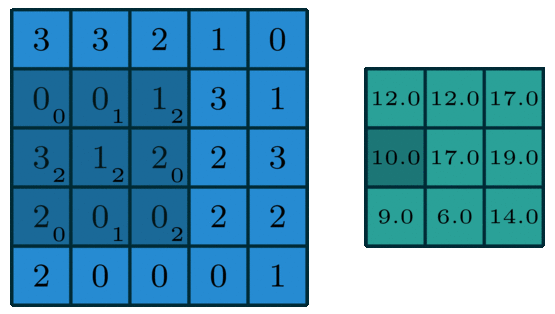
\includegraphics[width=0.6\linewidth]{convoliutional_pvz}
\caption{Konvoliucinio sluoksnio veikimo principas. Kairėje pusėje pradinių duomenų matrica, tamsiai mėlyna paryškinta zona, uždengta filtro branduoliu. Branduolio svoriai yra nurodyti kampuose. Dešinėje pusėje žalia matrica yra rezultatas, su paryškintu langeliu, kuris atitinka dabartinę branduolio poziciją.}
\label{fig:convoliutional_pvz}
\end{figure}

Kai yra gauta nauja matrica, ji yra praleidžiama pro aktyvacijos funkciją. Tai gali būti tiesinė, sigmoidės ar kitos formos funkcija, kuri veikia gautas reikšmes. Konvoliuciniams tinklams dažniausiai naudojama \emph{ReLU} funkcija. Tai yra netiesinė aktyvacijos funkcija: ji apdoroja gautą vektorių ir grąžina jo tikslią vertę, jei ji yra didesnė už nulį, priešingu atveju grąžina nulį. Jos formulė yra:
\begin{equation}
 g(z) = max\{0, z\}
\end{equation}

%Kad galutinės matricos dydis būtų toks pats, kaip pradinės matricos, yra naudojamas padidinimas (angl. \textit{padding}), tai yra papildomų reikšmių pridėjimas, \enquote{rėmelis} aplink duomenų matricos. Papildomos reikšmės dažniausiai yra nuliai.

Galutinio rezultato apdorojimui naudojama \emph{softmax} funkcija. Tai yra aktyvacijos funkcija, kuri yra naudojama klasifikacijos uždaviniuose: ji konvertuoja vektoriaus reikšmes į tikimybes, kurių suma yra lygi vienetui. Šios tikimybės yra skaičiuojamos taip: paimama reikšmės eksponentė ir normalizuojama naudojant visų reikšmių eksponenčių sumą:
\begin{equation}
P(y_{i} | x_{i}, W) = \frac{e^{f_{y_i}}}{\sum _j\cdot e^{f_j}}
\end{equation}

\subsubsection{Dirbtinio neuroninio tinklo apmokymas}

Mašininio mokymosi veikimo bendri etapai yra:
\begin{itemize} 
\item Didelės tikrų duomenų duombazės pasirinkimas: kuo daugiau duomenų ir kuo jie kokybiškesni bei apima daugiau galimų variantų, tuo geriau galima apmokinti funkciją.\cite{stepniewska-dziubinska_development_2018}
\item Duomenų dalijimas į apmokymo ir testavimo rinkinius (dažnai 70/30 ar 80/20 santykiu). Apmokymo rinkinys būna didesnis dėl to, kad apmokymui reikia kuo daugiau duomenų.
\item Funkcijos apmokymas naudojant tik apmokymo rinkinį: algoritmas keičia savo parametrus taip, kad kuo tiksliau atspėtų apmokymo duomenis, randa bendrus dėsningumus;
\item Funkcijos patikrinimas ant testavimo duomenų: jei atsiranda didelis procentas blogai prognozuotų reikšmių, reiškia funkcija yra permokyta (angl. \textit{overfitted}). Jei teisingai prognozuotų reikšmių procentas panašus į gautą po funkcijos apmokymo ir kartu pakankamai aukštas, funkcija yra paruošta naudojimui ar tolimesniam testavimui.
\end{itemize}

Visų parametrų reikšmių patikrinimas gali užtrukti itin didelį laiko kiekį, todėl yra taikoma gradientinio nusileidimo algoritmas (angl. \textit{stochastic gradient descent}). Jis gali būti apibendrintas kaip iteratyvinis algoritmas, kuris prasideda nuo atsitiktinio funkcijos taško ir žingsneliais juda žemiausio funkcijos taško link, kai funkcijos $x$ reikšmės yra pasirinkti svoriai, o $y$ reikšmės - skirtumas tarp tikrų duomenų ir prognozuoto rezultato, arba klaidos dydis. Taigi yra ieškoma mažiausio $y$, kas būtų mažiausiai klaidingas svorių rinkinys. Žingsnio dydis vadinamas mokymo greičiu (angl. \textit{learning rate}) ir paprastai žymimas $\eta$; kuo jis didesnis, tuo didesniai žingsniais juda algoritmas ir gali apsilenkti žemiausią tašką, todėl patartina rinktis mažesnį $\eta$.

Mašininio mokymosi algoritmai gali persimokyti.\cite{ragoza_proteinligand_2017} Tai reiškia, kad jie gerai prognozuos duomenis, su kuriais mokėsi, bet blogai prognozuos kitus duomenis iš tos pačios srities. Taip atsitinka, kai modeliui pateikti duomenys neapima visų galimų variantų. Pavyzdžiui, modelis gali prisitaikyti prie tam tikros baltymų šeimos ir blogai prognozuoti kitos baltymų šeimos sąryšį su ligandu. Kitaip sakant, modelis neišmoko tam tikrų taisyklių, bet tiesiog \enquote{iškalė} duomenis mintinai. Permokymą galima pastebėti, kai mokymosi rinkinio prognozavimas pavyksta kuo puikiausiai, tuo pačiu metu su nepriklausomais duomenimis prognozavimas tampa labai klaidingas. Modelis tampa specifinis.\cite{lehr_playing_2017} Tai galima taisyti keliais būdais, vienas iš kurių yra nežymiai pakeistų duomenų pridėjimas (angl. \textit{data augmentation}).\cite{ragoza_proteinligand_2017} Pakeitimai turi būti nereikšmingi, kad modelis nepradėtų mokytis ant klaidingų duomenų. Pavyzdžiui jei kalbama apie konvoliucinius neuroninius tinklus, galima tą patį paveiksliuką pasukti arba pridėti nežymaus triukšmo. Baltymų-ligandų kompleksų atveju, jei modelis mokosi iš kompleksų trimačių struktūrų, galima tas struktūras įvairiai pasukti. 

Kitas būdas kovoti su permokymu yra kryžminės kontrolės naudojimas (angl. \textit{cross-validation}).\cite{lehr_playing_2017}\cite{wojcikowski_performance_2017} Šiuo atveju duomenys dalinami į $k$ grupes. Toliau modelis mokosi naudojant $k-1$ grupių duomenis, o paskutinė grupė veikia kaip testavimo rinkinys. Šis procesas kartojasi $k$ kart, kiekvieną kartą išrenkama vis kita grupė testavimui. Taip įvyksta tolygus mokymasis su visais duomenimis.\cite{wojcikowski_performance_2017}

Nuostolių funkcijos reguliarizacija taip pat yra veiksmingas būdas mažinti permokymą. Pačios žinomiausios yra L1 ir L2 reguliarizacijos. L1 algoritmas (dar žinomas kaip Lasso regresija) tiesiogiai mažina parametrų svorius. Parametrai, kurie turi mažesnį svorį, visai išnyksta. Taip modelis įgyja kontrastą, nes daugiau išryškėja lemtingi parametrai; tai puikiai tinka klasifikacijos metu atrinkti reikšmingus parametrus. L2 algoritmas (dar žinomas kaip gūbrio regresija, angl. \textit{ridge regression}) mažina parametrų kvadratinius svorius. Tuomet visi svoriai mažėja tolygiai, modelis tampa labiau generalizuotas.\cite{stepniewska-dziubinska_development_2018}

%-------------------------------------------------
%       VIRTUALI ATRANKA, DUOMENYS
%-------------------------------------------------

\subsection{Ligandų virtuali atranka}

Ligando įvedimas į baltymą daugiausia yra naudojamas vaistų projektavime. Prijungimų palyginimas leidžia nustatyti, kaip sąveikaus įvairios molekulės, ir taip atrenkami ligandai, kurie tikimiausiai bus veiksmingi vaistai. Savaime suprantama, kad vienos kompiuterinės analizės neužtenka: kiekviena atrinkta molekulė bus tiriama \textit{in vitro}, taip pat kiekvienas vaistas turi praeiti klinikinius tyrimus. Programinės įrangos panaudojimas molekulių prijungime yra esminis, kai norima sumažinti tiriamų molekulių skaičių iš pradinės ligandų duombazės.\cite{pereira_boosting_2016} Šis procesas vadinamas virtualia atranka (angl. \textit{virtual screening}). 

Virtuali atranka gali vykti dviems būdais: tai gali būti ligandų atranka pagal jų fiziko--chemines savybes lyginant su jau žinomais aktyviais ligandais; arba ligandus galima atrinkti pagal jų trimates struktūras, kai receptoriaus struktūra taip pat yra nustatyta. Struktūra paremta virtuali atranka dažniau yra tikslesnė negu paremta tiesiog fiziko--cheminėmis ligandų savybėmis.\cite{pereira_boosting_2016}

\subsubsection{Mašininio mokymosi vertinimo funkcijos ir jų pavyzdžiai}
\label{sec:vertinimo_funkciju_pavyzdziai}

Kaip jau buvo minėta anksčiau, pagrindinis skirtumas tarp klasikinių ir mašininio mokymosi vertinimo sistemų yra jų galutinio algoritmo įgavimo būdas. Klasikinio metodo vertinimo sistema turi turėti teorinę bazę -- žmogaus išvestą formulę. Mašininio mokymosi vertinimo sistema įgauna savo funkcionalumą mokymosi metu, pati atranda dėsningumus ir supranta, į kuriuos molekulės duomenis reikia atkreipti dėmesį. Mašininio mokymosi metodas yra pagrįstas didelio duomenų kiekio nagrinėjimu ir vertinimo funkcijos išvedimu keičiant funkcijos parametrus iki tol, kol funkcija gali kuo tiksliau prognozuoti baltymo--ligando komplekso jungimąsi. 

Viena iš populiariausių ligando įvedimo į baltymą programų yra \enquote{Autodock Vina}\cite{trott_autodock_2010}, pristatyta 2010 metais. Ji yra nemokama ir viešai prieinama. Jos vertinimo funkcija yra dažniausiai priskiriama prie empirinių funkcijų tipo, tačiau jos autoriai teigia, kad ji yra daugiau pagrįsta mašininiu mokymusi. Šiandien \enquote{Autodock Vina} galima aptikti tokiose plačiai naudojamose programose, kaip \enquote{UCSF Chimera}, bei daugelyje mokslinių straipsnių.

Moderniausi vertinimo funkcijų modeliai yra kuriami naudojant dirbtinius neuroninius tinklus, tačiau puikiai veikia ir kiti mašininio mokymosi algoritmai, tokie kaip atsitiktinių miškų (angl. \textit{Random Forest}) ar atraminių vektorių mašinų (angl. \textit{Support--Vector Machines}) algoritmai. Pavyzdžiui, Wong et al. \cite{wong_predicting_2013} panaudojo atraminių vektorių mašinų algoritmą ligando įvedimui į baltymą. Šis algoritmas yra skirtas rasti $N-1$ dimensijų (kai yra $N$ savybių) hiperplaną - tai yra atskirti duomenų taškus į klasterius hiperplano pagalba. Wong savo metodui panaudojo 29 baltymo--ligando komplekso savybes, tokios kaip jungties energija, sekos konservatyvumas, atstumas tarp molekulių ir t.t. Taip buvo nustatyta, kurie iš išrinktų baltymų ertmių arba \enquote{kišenių} turi didžiausią tikimybę pririšti ligandus. Tais pačiais metais buvo sukurta panašaus veikimo vertinimo funkcija \enquote{ID-score}, kuri pagrįsta atraminių vektorių regresija ir kiekvienam kompleksui išskiria net 50 parametrų.\cite{li_id-score_2013} Atsitiktinių miškų algoritmas buvo naudojamas \enquote{RF-score} vertinimo funkcijoje, po kurios buvo sumodeliuotos \enquote{RF-score--2}, \enquote{RF-score--3} ir \enquote{RF-score--VS} funkcijos. Paskutinė jų yra iki šiol stiprus konkurentas neuroninio tinklo funkcijoms.\cite{wojcikowski_performance_2017}

Pagal Ain et al.,\cite{ain_machine-learning_2015} pirma dirbtinio neuroninio tinklo baltymo--ligando surišimo vertinimo funkcija buvo pristatyta 2008 metais. Konvoliuciniais neuroniniais tinklais paremtos vertinimo funkcijų pavyzdžiai yra \enquote{AtomNet} (2013)\cite{wallach_atomnet_2015}, \enquote{DeepVS} (2016)\cite{pereira_boosting_2016}, \enquote{Gnina} (2017)\cite{ragoza_proteinligand_2017} ir \enquote{Pafnucy} (2018)\cite{stepniewska-dziubinska_development_2018}. Šiame darbe yra akcentuojamas \enquote{DeepVS} modelis, ir jo algoritmas yra naudojamas šio darbo vertinimo funkcijos kūrimui. Jis buvo parinktas dėl jo aukšto įvertinimo palyginus su senesnėmis vertinimo funkcijomis bei aiškaus ir nuoseklaus aprašo. Taip pat ši vertinimo funkcija yra viešai prieinama adresu \url{https://github.com/JanainaCruz/DeepVS}. 

\subsubsection{Duomenų paruošimas pateikimui į modelį}

Mašininio mokymosi modeliui yra ypač svarbu paruošti didelį ir kokybišką duomenų rinkinį, šiuo atveju baltymo--ligando kompleksų rinkinį su nustatyta $K_{d}$ (tiksli reikšmė reikalinga norint spręsti regresijos užduotį, o klasifikacijos užduočiai užtenka binarinio indikatoriaus apie komplekso aktyvumą). Tokius rinkinius galima gauti iš skirtingų duombazių; vieni populiariausių yra \enquote{RCSB PDB}, \enquote{CSAR} ir t.t.\cite{ragoza_proteinligand_2017} Taip pat yra mažesnės duombazės, skirtos būtent proteino--ligando kompleksams ir jų vertinimo funkcijoms, tokios kaip \enquote{PDBbind}. Ligandų paieškai gali būti naudojama \enquote{ZINC}, komercinių ligandų duomenų bazė. 

Pieš modeliui apdorojant duomenis, pačius duomenis būtinai reikia tinkamai paruošti. Šiuo atveju reikia išrinkti molekulių (baltymų ir ligandų) užrašymo būdą. Dažnai tam yra naudojami savybių vektoriai (molekuliniai vektoriai, angl. \textit{fingerprints}).\cite{ballester_does_2014} Molekuliniai vektoriai yra skaičiais užrašytų savybių rinkiniai. Priklausomai nuo vektoriaus tipo, jis gali būti įvairaus ilgio ir nurodyti skirtingus parametrus. Yra svarbu, kad kiekvienas kompleksas būtų užrašytas tuo pačiu formatu. Vektoriaus dydis ir informacija įtakoja galutinio modelio apmokymo greitį ir efektyvumą, nes vienos savybės gali turėti įtakos surišimo prognozavimui, kai kitos tik sulėtins skaičiavimus. Ballester et al.\cite{ballester_does_2014} teigia, kad didelis cheminių savybių tikslumas nebūtinai generuoja tikslesnį rezultatą. Panašus efektas buvo pastebėtas Ragoza et al.\cite{ragoza_proteinligand_2017}

Kalbant apie ligando bei receptoriaus molekulių trimates struktūras, ligando įvedimui į baltymą pastarajam yra iškarpomas ir naudojamas aktyvusis centras proceso greitinimui. Paskui gautą trimatį molekulės gabaliuką galima išreikšti kaip keturmatį tensorių, kuris yra sudarytas iš taškų (atomų); kiekvienas taškas turi tris koordinates ir savybių vektorių. Jame užrašomas atomo tipas, hibridizacija, ryšių kiekiai, dalinis krūvis ir t.t.\cite{stepniewska-dziubinska_development_2018}

%http://tug.ctan.org/info/symbols/comprehensive/symbols-a4.pdf

%\begin{figure}[H]
%\centering 
%\includegraphics[width=0.55 \linewidth]{failo pavadinimas, galima be plėtinio}
%\caption{Užrašas po paveiksliuko.}
%\label{fig:bla}
%\end{figure}

%\begin{figure}[H]
%\centering 
%\subfloat[Užrašas po pirmo pav\label{fig:abba}]{\includegraphics[width=0.45 \linewidth]{pirmo failo pavadinimas}}
%\subfloat[Užrašas po antro pav\label{fig:baobab}]{\includegraphics[width=0.45 \linewidth]{antro failo pavadinimas}}
%\caption{Bendras užrašas}
%\label{fig:blabla}
%\end{figure}

% \ref{fig:} pav: \href{https://upload.wikimedia.org/wikipedia/commons/2/20/Illu_blood_cell_lineage.jpg}{Eritropoezės schema}

% !TEX root = referatas.tex

% Sutrumpinimai:
% ReLU - Rectified Linear Unit
% EEM - Electronegativity Equalization Method

\section{METODAI IR MODELIAVIMAI}

\subsection{Duomenų apie molekules surinkimas}

\TD{Pasirinkti ligandai. Pasirinkti 60 proteinai, su kuriais žinomos sąveikos su ligandais. Baltymai turi būti geros kokybės. Trumpai aprašyti baltymų svarbumą. Ligandai turi būti apie 50/50 gerų ir "blogų", geriau be dekojų, bet tikriausiai reikės}

% -----------------------------------------------------------------------------------

\subsection{Lingadų įvedimas į batymą}

Ligandų įvedimas į baltymą atliekamas naudojant \emph{LeDock} programą. Ji buvo pasirinkta todėl, kad parodė aukštus įvertinimus palyginus su kitomis šiam tikslui pritaikytomis programomis.\cite{} \emph{LeDock} naudoja vertinimo funkciją, kuri skaičiuoja komplekso surišimo stiprumą: %http://www.lephar.com/download/LeDock.pdf
\begin{equation}
\Delta G_{bind}=\alpha \sum_{i \in lig}\left(E_{i}^{vdw}+E_{i}^{hb}\right) \Theta\left(E_{c o}-E_{i}^{v d w}-E_{i}^{h b}\right)+\beta(r) \sum_{i \in lig} \sum_{j \in pro} \frac{q_{i} q_{j}}{r_{i j}}+\gamma E_{lig}^{\text {strain}}
\end{equation}
kur $E^{vdw}$ ir $E^{hb}$ yra atitinkamai Van der Valso ir vandenilinių ryšių energijų sumos, $\Theta$ yra \emph{Heaviside} funkcija, $E_{co}$ yra 'cutoff' \TD{?} energijos suma, $q$ yra dalinis atomo krūvis, $r$ - atstumas tarp atomų poros, $\alpha$, $\beta$ ir $\gamma$ yra empiriniai koeficientai.
\TD{jei jis skaičiuoja naudojant dalinius krūvius, kodėl paskui juos reikia vėl skaičiuot?? Atrodo aš baltymui skaičiuoju prieš dockingą krūvius, o ligandams ne? Aš juos konvertuoju iš sdf į mol2, ar nurodžiu kad dar paskaičiuotų krūvius?}
\TD{Naudojama programa - LeDock. Jai reikalinga baltymo stukrūra, ligando struktūra ir aktyvaus centro koordinates. Akt.c.: PDBsum. 30x30x30 A. Koordinačių konvertavimas LeDockui.} 

% -----------------------------------------------------------------------------------

\subsection{Kompleksų kodavimas ir duomenų padavimas neuroniniam tinklui}

Įvedami į neuronini tinklą duomenys yra vektorių rinkinio pavidalo. Kiekvienas vektorius turi informaciją apie ligando atomą, artimiausius du ligando atomus ir du baltymo atomus. Yra aprašomi atomų tipai (pvz. N, C), daliniai krūviai (slankiojančio kablelio skaičiais), atstumai tarp pirmojo atomo ir kitų atomų (slankiojančio kablelio neneigiamas skaičius; pirmasis atomas turės 0), bei aminorūgšties tipai, kuriai priklauso baltymo atomai (pvz. Gln). Atomų daliniai krūviai atvaizduoja elektronų pasiskirstymą molekulėje, kas nulemia molekulės tam tikras chemines savybes.
Kiekvienas kompleksas po ligando įvedimo į baltymą su \emph{LeDock} pagalba turi informaciją apie baltymo ir ligando atomų koordinates trimatėje erdvėje, bei atomų tipus, tačiau neturi informacijos apie atomų dalinius krūvius. Jie yra skaičiuojami naudojant \emph{OpenBabel} įrankį ir pasirenkant EEM algoritmą. % https://www.ncbi.nlm.nih.gov/pmc/articles/PMC3716427/ https://www.ncbi.nlm.nih.gov/pmc/articles/PMC4667495/
Jis buvo pasirinktas todėl, kad pagal \cite{} ir \cite{} straipsnius, EEM algoritmas skaičiuoja dalinius krūvius ypač aukštu tikslumu.

EEM skaičiuoja elektronegatyvumą kiekvienam atomui molekulėje pagal tokią formulę: %https://www.pamoc.it/kw_eem.html

\begin{equation}
\chi_{i}=\left(\chi_{i}^{\circ}+\Delta \chi_{i}\right)+2\left(\eta_{i}^{\circ}+\Delta \eta_{i}\right) q_{i}+k \sum_{i \neq j}^{N} \frac{q_{j}}{r_{i, j}}
\end{equation}
čia $\chi_{i}^{\circ}$ yra izoliuoto atomo $i$ elektronegatyvumas, $\Delta \chi_{i}$ yra jo patikslinimas turint omenyje atomo buvimą molekulėje; $\eta_{i}^{\circ}$ yra atomo kietumas; $q_{i}$ yra atomo krūvis; $k \sum_{i \neq j}^{N} \frac{q_{j}}{r_{i, j}}$ parodo elektrostatinius santykius tarp šio atomo ir kiekvieno kito atomo $j$ molekulėje.

Tuomet bendras molekulės krūvis yra: 

\begin{equation}
Q=\sum_{i=1}^{N} q_{i}
\end{equation}



%ir taikant Gasteigerio algoritmą. Skaičiuojant $Q_i$ dalinį krūvį $i$ atomui, yra tokia formulė\cite{gasteiger_new_1978}:

%\begin{equation}
%Q_{i}=\sum_{a}\left\{\left[\sum_{j} \frac{1}{D_{i}}\left(x_{j}-x_{i}\right)+\sum_{k} \frac{1}{D_{k}}\left(x_{k}-x_{i}\right)\right]\left(\frac{1}{f}\right)^{a-1}\right\}
%\end{equation}
%kur $j$ ir $k$ yra šalia esantys atomai, kurie turi didesnį ar mažesnį elektronegatyvumą; $x_i$, $x_j$ ir $x_k$ yra atitinkamų atomų eletronegatyvumai; $D_i$ yra maksimalus elektronegatyvumo skirtumas, $a$ -- ?, $f$ -- ?


\TD{docking\_data\_processor, aprašyti}

% -----------------------------------------------------------------------------------

\subsection{Neuroninio tinklo architektūra}

%Neuroninis tinklas sudarytas iš daugelio neuronų. Kiekvienas neuronas gauna kelias įvestis, kiekviena iš kurių turi savo svorį. Iš pradžių svorio reikšmės yra parenkamos atsitiktiniu būdu, tačiau keičiamos modeliui besimokant. Neurono produkto skaičiavimo formulė atrodo taip:
%\begin{equation}
%z=\sum_{j=1}^{k} x_{j} w_{k}+b w_{0}
%\end{equation}
%kur $w_k$ yra tam tikros įvesties svoris ir $b$ yra nuolydis (angl. \textit{bias}). Nuolydis yra papildoma įvestis, kurios reikšmė yra fiksuota. Jis yra svarbus modelio lankstumui.

Pradinis neuroninio tinklo kodas yra paimtas iš \cite{pereira_boosting_2016}. Jis yra parašytas \emph{Python} 2.7 programavimo kalba. Šiam darbui jis buvo nežymiai pakeistas, kad atitiktų \emph{Python} 3.7 versijai. Taip pat šio kodo duomenų apdorojimo dalis yra pritaikyta darbui su \emph{Autodock Vina} programos failais, todėl buvo perrašyta tam, kad tiktų darbui su \emph{LeDock} programa. Šis neuroninis tinklas yra pavadintas \emph{DeepVS}. Jis yra konvoliucinis neuroninis tinklas ir operuoja su vektoriais. Tam jis naudoja tiesinį transformavimą, \emph{ReLU}  aktyvacijos funkciją ir \emph{dropout} reguliarizacijos metodą. \emph{Dropout} metodas yra atsitiktinių reikšmių išmetimas (atsitiktinių neuronų išjungimas), kas gerai veikia prieš modelio persimokymą. \emph{DeepVS} naudoja \emph{dropout} metodą su 0,5 tikimybe kiekvienai iš reikšmių būti išmestai. Gale yra taikoma \emph{softmax} funkcija, po kurios gaunamas galutinis baltymo--ligando komplekso įvertinimas.

%http://tug.ctan.org/info/symbols/comprehensive/symbols-a4.pdf

%\begin{figure}[H]
%\centering 
%\includegraphics[width=0.55 \linewidth]{failo pavadinimas, galima be plėtinio}
%\caption{Užrašas po paveiksliuko.}
%\label{fig:bla}
%\end{figure}

%\begin{figure}[H]
%\centering 
%\subfloat[Užrašas po pirmo pav\label{fig:abba}]{\includegraphics[width=0.45 \linewidth]{pirmo failo pavadinimas}}
%\subfloat[Užrašas po antro pav\label{fig:baobab}]{\includegraphics[width=0.45 \linewidth]{antro failo pavadinimas}}
%\caption{Bendras užrašas}
%\label{fig:blabla}
%\end{figure}

% \ref{fig:} pav: \href{https://upload.wikimedia.org/wikipedia/commons/2/20/Illu_blood_cell_lineage.jpg}{Eritropoezės schema}

\bibliographystyle{vgtu_darbas}
\addcontentsline{toc}{section}{LITERATŪRA} % kad literatūra būtų pridėta į table of contents
\bibliography{bakalaurinis}

\end{document}